% Options for packages loaded elsewhere
\PassOptionsToPackage{unicode}{hyperref}
\PassOptionsToPackage{hyphens}{url}
%
\documentclass[
  8pt,
  ignorenonframetext,
]{beamer}
\usepackage{pgfpages}
\setbeamertemplate{caption}[numbered]
\setbeamertemplate{caption label separator}{: }
\setbeamercolor{caption name}{fg=normal text.fg}
\beamertemplatenavigationsymbolsempty
% Prevent slide breaks in the middle of a paragraph
\widowpenalties 1 10000
\raggedbottom
\setbeamertemplate{part page}{
  \centering
  \begin{beamercolorbox}[sep=16pt,center]{part title}
    \usebeamerfont{part title}\insertpart\par
  \end{beamercolorbox}
}
\setbeamertemplate{section page}{
  \centering
  \begin{beamercolorbox}[sep=12pt,center]{part title}
    \usebeamerfont{section title}\insertsection\par
  \end{beamercolorbox}
}
\setbeamertemplate{subsection page}{
  \centering
  \begin{beamercolorbox}[sep=8pt,center]{part title}
    \usebeamerfont{subsection title}\insertsubsection\par
  \end{beamercolorbox}
}
\AtBeginPart{
  \frame{\partpage}
}
\AtBeginSection{
  \ifbibliography
  \else
    \frame{\sectionpage}
  \fi
}
\AtBeginSubsection{
  \frame{\subsectionpage}
}
\usepackage{amsmath,amssymb}
\usepackage{lmodern}
\usepackage{ifxetex,ifluatex}
\ifnum 0\ifxetex 1\fi\ifluatex 1\fi=0 % if pdftex
  \usepackage[T1]{fontenc}
  \usepackage[utf8]{inputenc}
  \usepackage{textcomp} % provide euro and other symbols
\else % if luatex or xetex
  \usepackage{unicode-math}
  \defaultfontfeatures{Scale=MatchLowercase}
  \defaultfontfeatures[\rmfamily]{Ligatures=TeX,Scale=1}
\fi
% Use upquote if available, for straight quotes in verbatim environments
\IfFileExists{upquote.sty}{\usepackage{upquote}}{}
\IfFileExists{microtype.sty}{% use microtype if available
  \usepackage[]{microtype}
  \UseMicrotypeSet[protrusion]{basicmath} % disable protrusion for tt fonts
}{}
\makeatletter
\@ifundefined{KOMAClassName}{% if non-KOMA class
  \IfFileExists{parskip.sty}{%
    \usepackage{parskip}
  }{% else
    \setlength{\parindent}{0pt}
    \setlength{\parskip}{6pt plus 2pt minus 1pt}}
}{% if KOMA class
  \KOMAoptions{parskip=half}}
\makeatother
\usepackage{xcolor}
\IfFileExists{xurl.sty}{\usepackage{xurl}}{} % add URL line breaks if available
\IfFileExists{bookmark.sty}{\usepackage{bookmark}}{\usepackage{hyperref}}
\hypersetup{
  hidelinks,
  pdfcreator={LaTeX via pandoc}}
\urlstyle{same} % disable monospaced font for URLs
\newif\ifbibliography
\usepackage{color}
\usepackage{fancyvrb}
\newcommand{\VerbBar}{|}
\newcommand{\VERB}{\Verb[commandchars=\\\{\}]}
\DefineVerbatimEnvironment{Highlighting}{Verbatim}{commandchars=\\\{\}}
% Add ',fontsize=\small' for more characters per line
\usepackage{framed}
\definecolor{shadecolor}{RGB}{248,248,248}
\newenvironment{Shaded}{\begin{snugshade}}{\end{snugshade}}
\newcommand{\AlertTok}[1]{\textcolor[rgb]{0.94,0.16,0.16}{#1}}
\newcommand{\AnnotationTok}[1]{\textcolor[rgb]{0.56,0.35,0.01}{\textbf{\textit{#1}}}}
\newcommand{\AttributeTok}[1]{\textcolor[rgb]{0.77,0.63,0.00}{#1}}
\newcommand{\BaseNTok}[1]{\textcolor[rgb]{0.00,0.00,0.81}{#1}}
\newcommand{\BuiltInTok}[1]{#1}
\newcommand{\CharTok}[1]{\textcolor[rgb]{0.31,0.60,0.02}{#1}}
\newcommand{\CommentTok}[1]{\textcolor[rgb]{0.56,0.35,0.01}{\textit{#1}}}
\newcommand{\CommentVarTok}[1]{\textcolor[rgb]{0.56,0.35,0.01}{\textbf{\textit{#1}}}}
\newcommand{\ConstantTok}[1]{\textcolor[rgb]{0.00,0.00,0.00}{#1}}
\newcommand{\ControlFlowTok}[1]{\textcolor[rgb]{0.13,0.29,0.53}{\textbf{#1}}}
\newcommand{\DataTypeTok}[1]{\textcolor[rgb]{0.13,0.29,0.53}{#1}}
\newcommand{\DecValTok}[1]{\textcolor[rgb]{0.00,0.00,0.81}{#1}}
\newcommand{\DocumentationTok}[1]{\textcolor[rgb]{0.56,0.35,0.01}{\textbf{\textit{#1}}}}
\newcommand{\ErrorTok}[1]{\textcolor[rgb]{0.64,0.00,0.00}{\textbf{#1}}}
\newcommand{\ExtensionTok}[1]{#1}
\newcommand{\FloatTok}[1]{\textcolor[rgb]{0.00,0.00,0.81}{#1}}
\newcommand{\FunctionTok}[1]{\textcolor[rgb]{0.00,0.00,0.00}{#1}}
\newcommand{\ImportTok}[1]{#1}
\newcommand{\InformationTok}[1]{\textcolor[rgb]{0.56,0.35,0.01}{\textbf{\textit{#1}}}}
\newcommand{\KeywordTok}[1]{\textcolor[rgb]{0.13,0.29,0.53}{\textbf{#1}}}
\newcommand{\NormalTok}[1]{#1}
\newcommand{\OperatorTok}[1]{\textcolor[rgb]{0.81,0.36,0.00}{\textbf{#1}}}
\newcommand{\OtherTok}[1]{\textcolor[rgb]{0.56,0.35,0.01}{#1}}
\newcommand{\PreprocessorTok}[1]{\textcolor[rgb]{0.56,0.35,0.01}{\textit{#1}}}
\newcommand{\RegionMarkerTok}[1]{#1}
\newcommand{\SpecialCharTok}[1]{\textcolor[rgb]{0.00,0.00,0.00}{#1}}
\newcommand{\SpecialStringTok}[1]{\textcolor[rgb]{0.31,0.60,0.02}{#1}}
\newcommand{\StringTok}[1]{\textcolor[rgb]{0.31,0.60,0.02}{#1}}
\newcommand{\VariableTok}[1]{\textcolor[rgb]{0.00,0.00,0.00}{#1}}
\newcommand{\VerbatimStringTok}[1]{\textcolor[rgb]{0.31,0.60,0.02}{#1}}
\newcommand{\WarningTok}[1]{\textcolor[rgb]{0.56,0.35,0.01}{\textbf{\textit{#1}}}}
\setlength{\emergencystretch}{3em} % prevent overfull lines
\providecommand{\tightlist}{%
  \setlength{\itemsep}{0pt}\setlength{\parskip}{0pt}}
\setcounter{secnumdepth}{-\maxdimen} % remove section numbering
% type setting
% ------------------------------------------------------------------------------
\usepackage[german]{babel}     

% fonts
% ------------------------------------------------------------------------------
\usefonttheme{professionalfonts}

% slide title and horizontal line
% ------------------------------------------------------------------------------
\setbeamertemplate{frametitle}{%
    \vskip-30pt \color{black}\large%
    \begin{minipage}[b][23pt]{120mm}%
    \flushleft\insertframetitle%
    \end{minipage}%
}

\setbeamertemplate{headline}										
{
\vskip10pt\hfill\hspace{3.5mm} 										 
\vskip15pt\color{black}\rule{\textwidth}{0.4pt} 					 
}

% slide number
% ---------------------------------------------------------------
\setbeamertemplate{navigation symbols}{}
\setbeamertemplate{footline}
{
\vskip5pt
\vskip2pt
\makebox[123mm]{\hspace{7.5mm}
\hfill Programmierung und Deskriptive Statistik $\vert$ 
\copyright $ $ 2022 Dirk Ostwald CC BY-NC-SA 4.0 $\vert$ 
Folie \insertframenumber}
\vskip4pt
}

% block color scheme
% ------------------------------------------------------------------------------
% colors
\definecolor{white}{RGB}{255,255,255}
\definecolor{grey}{RGB}{235,235,235}
\definecolor{lightgrey}{RGB}{245,245,245}
\definecolor{LightBlue}{RGB}{220,220,255}
\definecolor{darkblue}{RGB}{51, 51, 153}

% definitions and theorems
\setbeamercolor{block title}{fg = black, bg = grey}
\setbeamercolor{block body}{fg = black, bg = lightgrey}

% general line spacing 
% ------------------------------------------------------------------------------
\linespread{1.3}

% local line spacing
% ------------------------------------------------------------------------------
\usepackage{setspace}

% colors
% -----------------------------------------------------------------------------
\usepackage{color}

% justified text
% ------------------------------------------------------------------------------
\usepackage{ragged2e}
\usepackage{etoolbox}
\apptocmd{\frame}{}{\justifying}{}

% bullet point lists
% -----------------------------------------------------------------------------
\setbeamertemplate{itemize item}[circle]
\setbeamertemplate{itemize subitem}[circle]
\setbeamertemplate{itemize subsubitem}[circle]
\setbeamercolor{itemize item}{fg = black}
\setbeamercolor{itemize subitem}{fg = black}
\setbeamercolor{itemize subsubitem}{fg = black}
\setbeamercolor{enumerate item}{fg = black}
\setbeamercolor{enumerate subitem}{fg = black}
\setbeamercolor{enumerate subsubitem}{fg = black}
\setbeamerfont{itemize/enumerate body}{}
\setbeamerfont{itemize/enumerate subbody}{size = \normalsize}
\setbeamerfont{itemize/enumerate subsubbody}{size = \normalsize}

% color links
% ------------------------------------------------------------------------------
\usepackage{hyperref}
\definecolor{urls}{RGB}{204,0,0}
\hypersetup{colorlinks, citecolor = darkblue, urlcolor = urls}


% additional math commands
% ------------------------------------------------------------------------------
\usepackage{bm}                                         % bold math symbols
\newcommand{\niton}{\not\owns}

% text highlighting
% ------------------------------------------------------------------------------
\usepackage{soul}
\makeatletter
\let\HL\hl
\renewcommand\hl{%
  \let\set@color\beamerorig@set@color
  \let\reset@color\beamerorig@reset@color
  \HL}
\makeatother

% equation highlighting
% -----------------------------------------------------------------------------
\newcommand{\highlight}[2][yellow]{\mathchoice%
  {\colorbox{#1}{$\displaystyle#2$}}%
  {\colorbox{#1}{$\textstyle#2$}}%
  {\colorbox{#1}{$\scriptstyle#2$}}%
  {\colorbox{#1}{$\scriptscriptstyle#2$}}}%

% additional mathematical operators
% ------------------------------------------------------------------------------
\DeclareMathOperator*{\argmax}{arg\,max}
\DeclareMathOperator*{\argmin}{arg\,min}

\ifluatex
  \usepackage{selnolig}  % disable illegal ligatures
\fi
\newlength{\cslhangindent}
\setlength{\cslhangindent}{1.5em}
\newlength{\csllabelwidth}
\setlength{\csllabelwidth}{3em}
\newenvironment{CSLReferences}[2] % #1 hanging-ident, #2 entry spacing
 {% don't indent paragraphs
  \setlength{\parindent}{0pt}
  % turn on hanging indent if param 1 is 1
  \ifodd #1 \everypar{\setlength{\hangindent}{\cslhangindent}}\ignorespaces\fi
  % set entry spacing
  \ifnum #2 > 0
  \setlength{\parskip}{#2\baselineskip}
  \fi
 }%
 {}
\usepackage{calc}
\newcommand{\CSLBlock}[1]{#1\hfill\break}
\newcommand{\CSLLeftMargin}[1]{\parbox[t]{\csllabelwidth}{#1}}
\newcommand{\CSLRightInline}[1]{\parbox[t]{\linewidth - \csllabelwidth}{#1}\break}
\newcommand{\CSLIndent}[1]{\hspace{\cslhangindent}#1}

\author{}
\date{\vspace{-2.5em}}

\begin{document}

\begin{frame}[plain]{}
\protect\hypertarget{section}{}
\center

\begin{center}
\includegraphics[width=0.2\linewidth]{2_Abbildungen/pds_2_otto} \end{center}

\vspace{2mm}

\huge

Programmierung und Deskriptive Statistik \vspace{6mm}

\large

BSc Psychologie WiSe 2021/22

\vspace{6mm}
\large

Prof.~Dr.~Dirk Ostwald
\end{frame}

\begin{frame}{Formalia}
\protect\hypertarget{formalia}{}
Modul A2 Einführung in die Forschungsmethoden der Psychologie

\begin{itemize}
\tightlist
\item
  Donnerstags 7.00 - 9.00 Uhr G22A-H2 (Volksbankhörsaal)
\item
  Traditioneller, wenig sinnvoller Kurs
\item
  Sinnvoller, neu überarbeiteter Kurs im Sommersemester 2022
\end{itemize}

Modul C2 Computergestützte Datenanalyse

\begin{itemize}
\tightlist
\item
  Donnerstags 15.00 - 17.00 Uhr G40-H231 (hier und jetzt)
\item
  Bearbeitung im WiSe 2021/22 empfohlen
\end{itemize}

Klausuren A2 und C2 werden sowohl im WiSe 21/22 als auch im SoSe 22
angeboten

Klausurvoraussetzung C2 nach Studienordnung erfolgreicher Abschluss von
C1
\end{frame}

\begin{frame}[plain]{}
\protect\hypertarget{section-1}{}
\vfill
\huge
\begin{center}
(2) R und RStudio Grundlagen
\end{center}
\vfill
\end{frame}

\begin{frame}{}
\protect\hypertarget{section-2}{}
\large
\vfill
\setstretch{2}

R und RStudio

Arithmetik, Logik und Präzedenz

Variablen

Datenstrukturen

Übungen und Selbstkontrollfragen
\end{frame}

\begin{frame}{}
\protect\hypertarget{section-3}{}
\large
\vfill
\setstretch{2}

\textbf{R und RStudio}

Arithmetik, Logik und Präzedenz

Variablen

Datenstrukturen

Übungen und Selbstkontrollfragen
\end{frame}

\begin{frame}{R und RStudio}
\protect\hypertarget{r-und-rstudio}{}
\setstretch{1.6}
\large

\textcolor{darkblue}{Was ist R?}

\normalsize

Eine Programmiersprache und ein Softwarepaket.

Entwickelt von Ihaka and Gentleman (1996).

Freier Dialekt der propietären Software S (Becker, Chambers, and Wilks
(1988)).

Weiterentwickelt und gepflegt durch
\href{https://www.r-project.org/contributors.html}{R Core Team} und
\href{https://www.r-project.org/foundation/}{R Foundation}

Interpretierte imperativ-objektorientierte 4GL Sprache.

Optimiert und populär für statistische Datenanalysen.

Große Community mit etwa 20.000 beigetragenen R Paketen (Erweiterungen)

Evolviert und konservativ im Kern, konsistent und progressiv in
\href{https://cran.r-project.org/web/packages/}{R Paketen}.
\end{frame}

\begin{frame}{R und RStudio}
\protect\hypertarget{r-und-rstudio-1}{}
\large

\textcolor{darkblue}{Wie bekommt man R?} \normalsize

Runterladen (z.B. \url{https://cran.r-project.org/bin/windows/base/})
und installieren. \vspace{2mm}

\begin{center}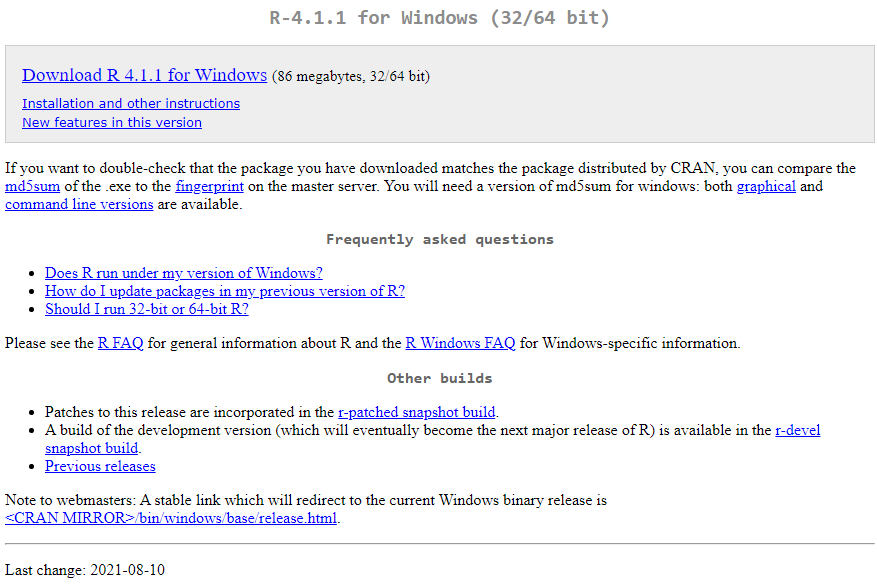
\includegraphics[width=0.8\linewidth]{2_Abbildungen/pds_2_r_download} \end{center}
\end{frame}

\begin{frame}{R und RStudio}
\protect\hypertarget{r-und-rstudio-2}{}
\setstretch{1.5}
\large

\textcolor{darkblue}{Was kann man mit R machen?} \normalsize

Datensätze laden, manipulieren, und speichern.

Eine Vielzahl von Berechnungen an verschiedenen Datenstrukturen
durchführen.

Eine Vielzahl statistischer Analyse Methoden auf Daten anwenden.

Datenanalyseskripte schreiben und Abbildungen generieren.

Präsentationen \href{https://bookdown.org/yihui/rmarkdown/}{RMarkdown}
und Bücher \href{https://bookdown.org/yihui/bookdown/}{RBookdown}
erstellen.

\vspace{2mm}

\large

\textcolor{darkblue}{Was kann man mit R (bisher) nicht so gut machen?}
\normalsize

In einer ansprechenden Umgebung programmieren (\(\Rightarrow\) RStudio).

Scientific Computing (\(\Rightarrow\) Python, Matlab, Julia).

Psychologische Experimente programmieren (\(\Rightarrow\) Python,
Matlab)
\end{frame}

\begin{frame}[fragile]{R und RStudio}
\protect\hypertarget{r-und-rstudio-3}{}
\large

\textcolor{darkblue}{Wie bekommt man Hilfe zu R?} \normalsize

Googlen

\url{https://stackoverflow.com/}

Während der Programmierung und bei bekanntem Funktionsnamen

\begin{Shaded}
\begin{Highlighting}[]
\NormalTok{?mean}
\FunctionTok{help}\NormalTok{(mean)}
\end{Highlighting}
\end{Shaded}

Für längere Tutorials

\begin{Shaded}
\begin{Highlighting}[]
\FunctionTok{browseVignettes}\NormalTok{()}
\end{Highlighting}
\end{Shaded}

\url{https://rseek.org/}

\url{https://www.rstudio.com/resources/cheatsheets/}

\url{https://www.r-bloggers.com/}
\end{frame}

\begin{frame}{R und RStudio}
\protect\hypertarget{r-und-rstudio-4}{}
\setstretch{1.6}
\large

\textcolor{darkblue}{Was ist RStudio?} \normalsize

Eine Softwareentwicklungsumgebung für R

Softwareentwicklungsumgebung = Integrated Development Environment

IDEs sind Programme zum Programmieren mit einer Programmiersprache

Kommandozeile, Skripteditor, Vielzahl weiterer Tools

Freemium Produkt von RStudio, Inc.~(IDE frei, Server kostenpflichtig)

Initial Release 2011, Affero General Public License

Keine Verbindung zu R Core Team oder R Foundation
\end{frame}

\begin{frame}{R und RStudio}
\protect\hypertarget{r-und-rstudio-5}{}
\large

\textcolor{darkblue}{Wie bekommt man RStudio?} \vspace{1mm}

Runterladen (\url{https://www.rstudio.com/products/rstudio/}) und
installieren \vspace{2mm}

\begin{center}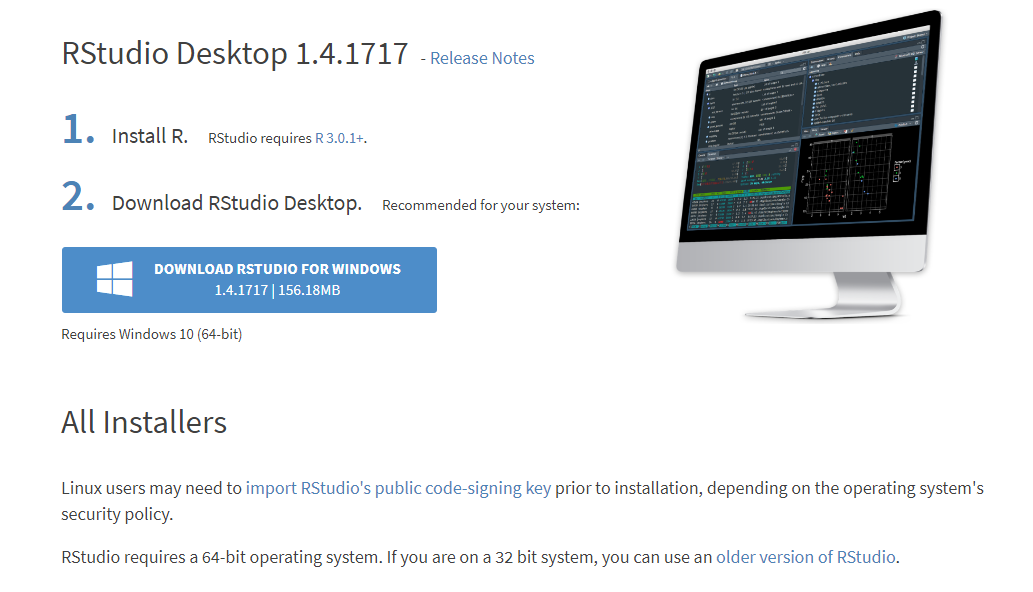
\includegraphics[width=0.8\linewidth]{2_Abbildungen/pds_2_rstudio_download} \end{center}
\end{frame}

\begin{frame}{R und RStudio}
\protect\hypertarget{r-und-rstudio-6}{}
\setstretch{1.6}
\vspace{2mm}
\large

\textcolor{darkblue}{Was kann man mit RStudio machen?} \normalsize

R Skripte erzeugen, bearbeiten, und laufen lassen

R Skripte in R Projekten organisieren

Laut Eigenwerbung

\small

\begin{itemize}
\tightlist
\item
  Access RStudio locally
\item
  Syntax highlighting, code completion, and smart indentation
\item
  Execute R code directly from the source editor
\item
  Quickly jump to function definitions
\item
  View content changes in real-time with the Visual Markdown Editor
\item
  Easily manage multiple working directories using projects
\item
  Integrated R help and documentation
\item
  Interactive debugger to diagnose and fix errors
\item
  Extensive package development tools
\end{itemize}
\end{frame}

\begin{frame}{R und RStudio}
\protect\hypertarget{r-und-rstudio-7}{}
\large

\textcolor{darkblue}{Was kann man mit RStudio machen?} \normalsize

Custom Layout via Tools \(\rightarrow\) Global Options \ldots{}

\begin{center}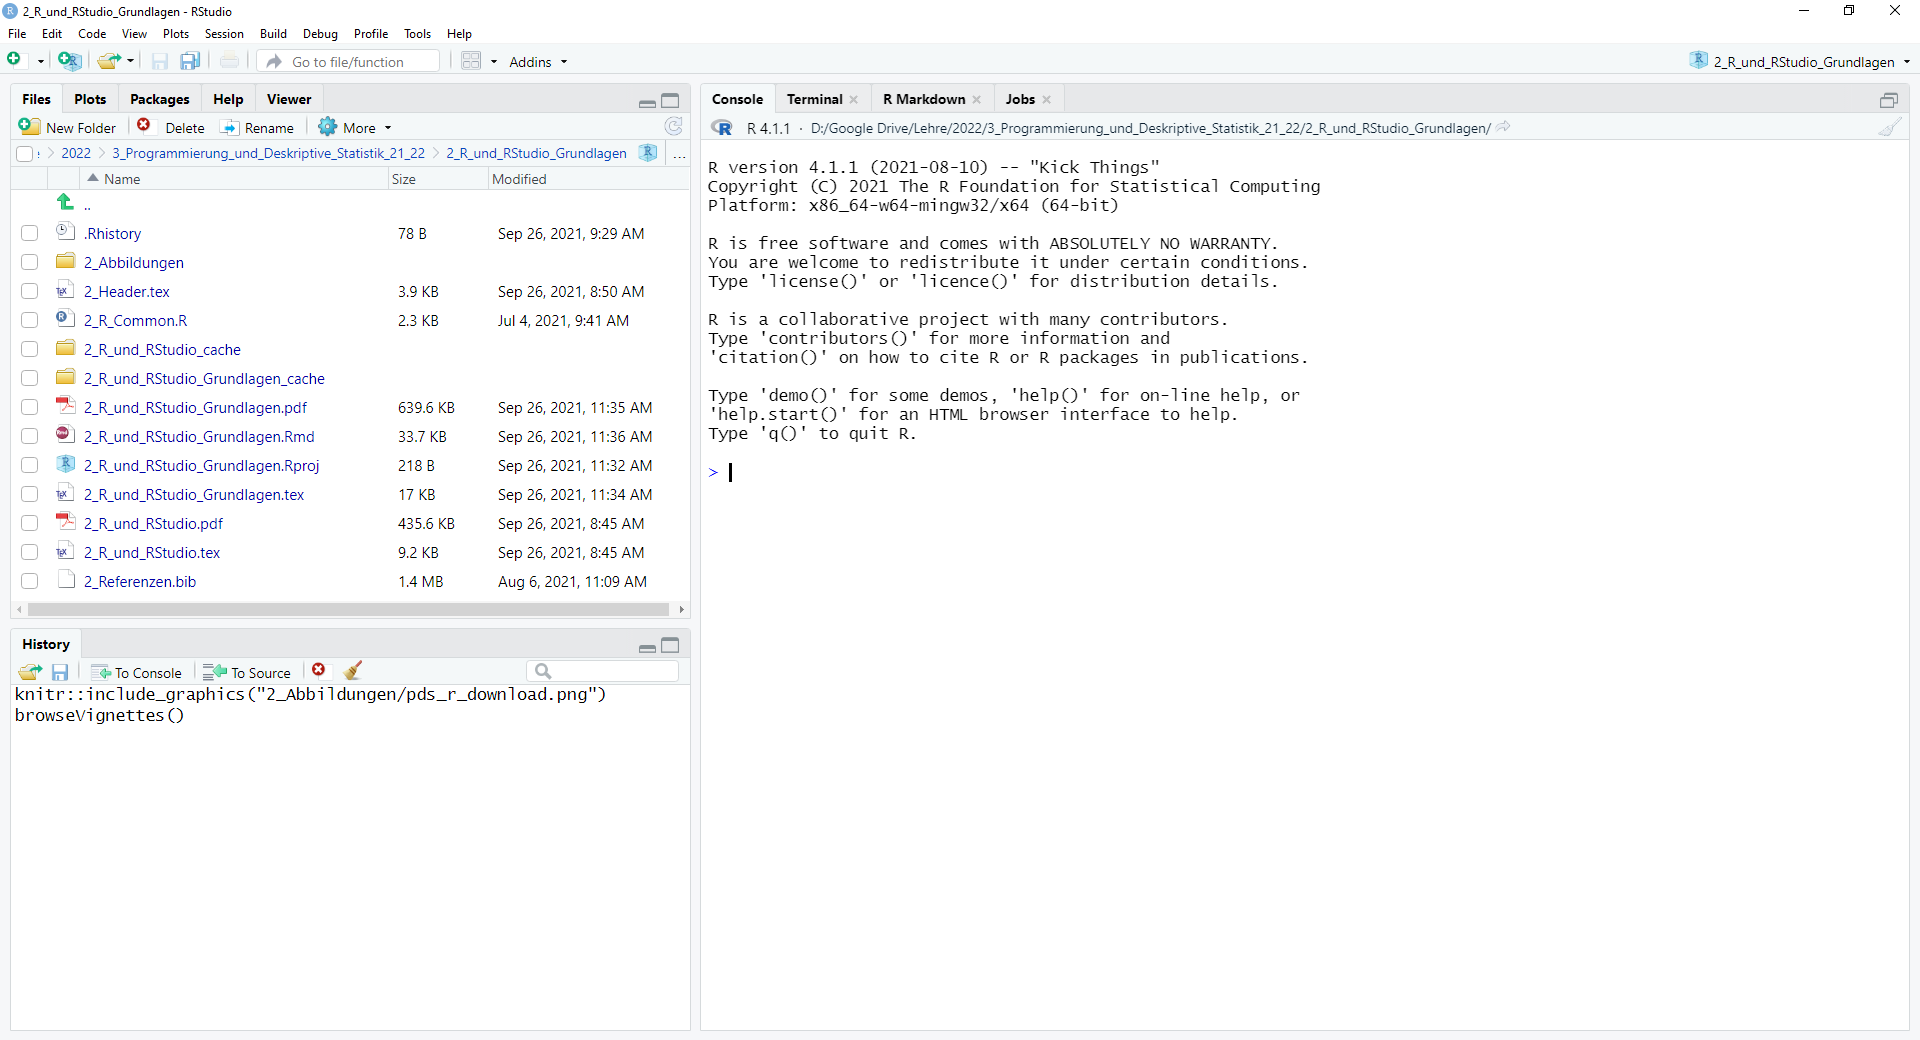
\includegraphics[width=0.9\linewidth]{2_Abbildungen/pds_2_rstudio} \end{center}
\end{frame}

\begin{frame}{R und RStudio}
\protect\hypertarget{r-und-rstudio-8}{}
\large

\textcolor{darkblue}{Wie bekommt man Hilfe zu RStudio?}

\normalsize

Googlen

Zur Einführung \(\Rightarrow\)
\href{https://support.rstudio.com/hc/en-us/sections/200107586-Using-the-RStudio-IDE}{Using
the RStudio IDE}

\begin{center}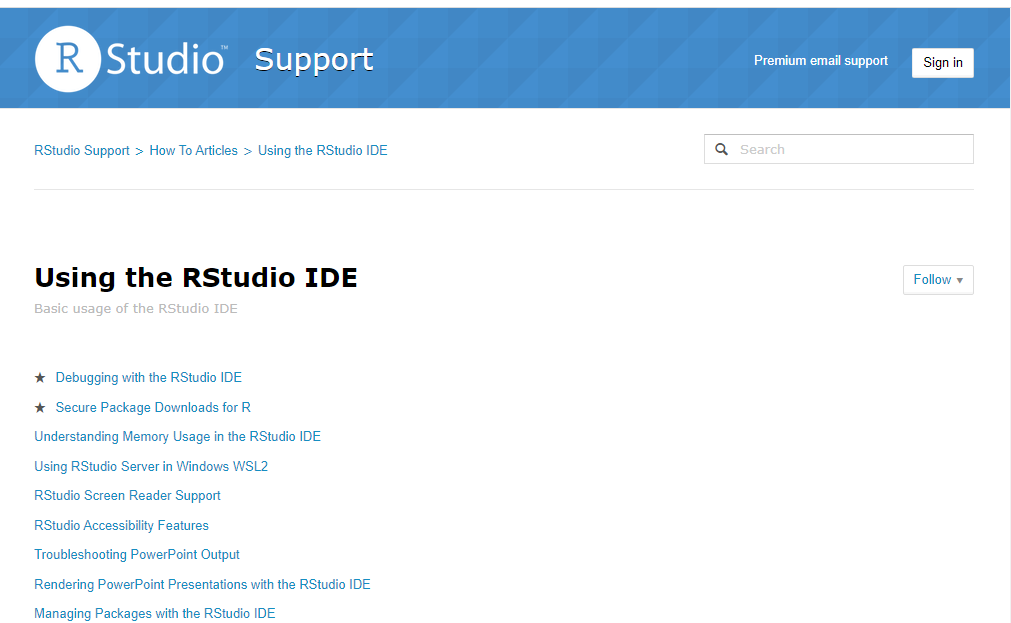
\includegraphics[width=0.7\linewidth]{2_Abbildungen/pds_2_using_rstudio} \end{center}
\end{frame}

\begin{frame}[fragile]{R und RStudio}
\protect\hypertarget{r-und-rstudio-9}{}
\setstretch{1.7}
\large

\textcolor{darkblue}{R Kommandozeile $\vert$ Working in the Console}
\normalsize

Eingabe von R Befehlen bei \(>\)

Autocomplete mit Tab

Vorherige Befehle mit Cursor \(\uparrow\)

Bereinigen des Konsolenoutputs mit Ctrl + L

Code Ausführungsstopp mit Esc

\begin{Shaded}
\begin{Highlighting}[]
\FunctionTok{print}\NormalTok{(}\StringTok{"Hallo Welt!"}\NormalTok{)}
\end{Highlighting}
\end{Shaded}

\begin{verbatim}
> [1] "Hallo Welt!"
\end{verbatim}

\textbf{Code-Snippets in diesen Folien immer aktiv in der Konsole
nachvollziehen!}
\end{frame}

\begin{frame}[fragile]{R und RStudio}
\protect\hypertarget{r-und-rstudio-10}{}
\setstretch{1.4}
\large

\textcolor{darkblue}{R Skripte $\vert$ Executing and Editing Code}
\small

File \(\rightarrow\) New File \(\rightarrow\) R Script oder Ctrl + Shift
+ N für neue .R Datei

Open File oder Ctrl + O zum Öffnen bestehender .R Datei

Eintippen von

\begin{Shaded}
\begin{Highlighting}[]
\FunctionTok{print}\NormalTok{(}\StringTok{"Hallo Welt!"}\NormalTok{)  }\CommentTok{\# Hinter Hashtags stehen dokumentierende Kommentare}
\FunctionTok{print}\NormalTok{(}\StringTok{"Hallo R!"}\NormalTok{)     }\CommentTok{\# Kommentare werden nicht ausgefuehrt}
\end{Highlighting}
\end{Shaded}

Ausführen der einzelnen Zeile, auf welcher der Cursor ruht

\(\Rightarrow\) Run oder Ctrl + Enter

Ausführen aller Zeilen

\(\Rightarrow\) Source oder Ctrl + Shift + Enter oder

\(\Rightarrow\) Tickmark bei Source on Save setzen und Ctrl + S

\textbf{Code-Snippets in diesen Folien immer aktiv in einem R Skript
dokumentieren!}
\end{frame}

\begin{frame}{R und RStudio}
\protect\hypertarget{r-und-rstudio-11}{}
\setstretch{1.4}
\large

\textcolor{darkblue}{Das R und RStudio Data Science Universum}
\vspace{2mm}

\begin{center}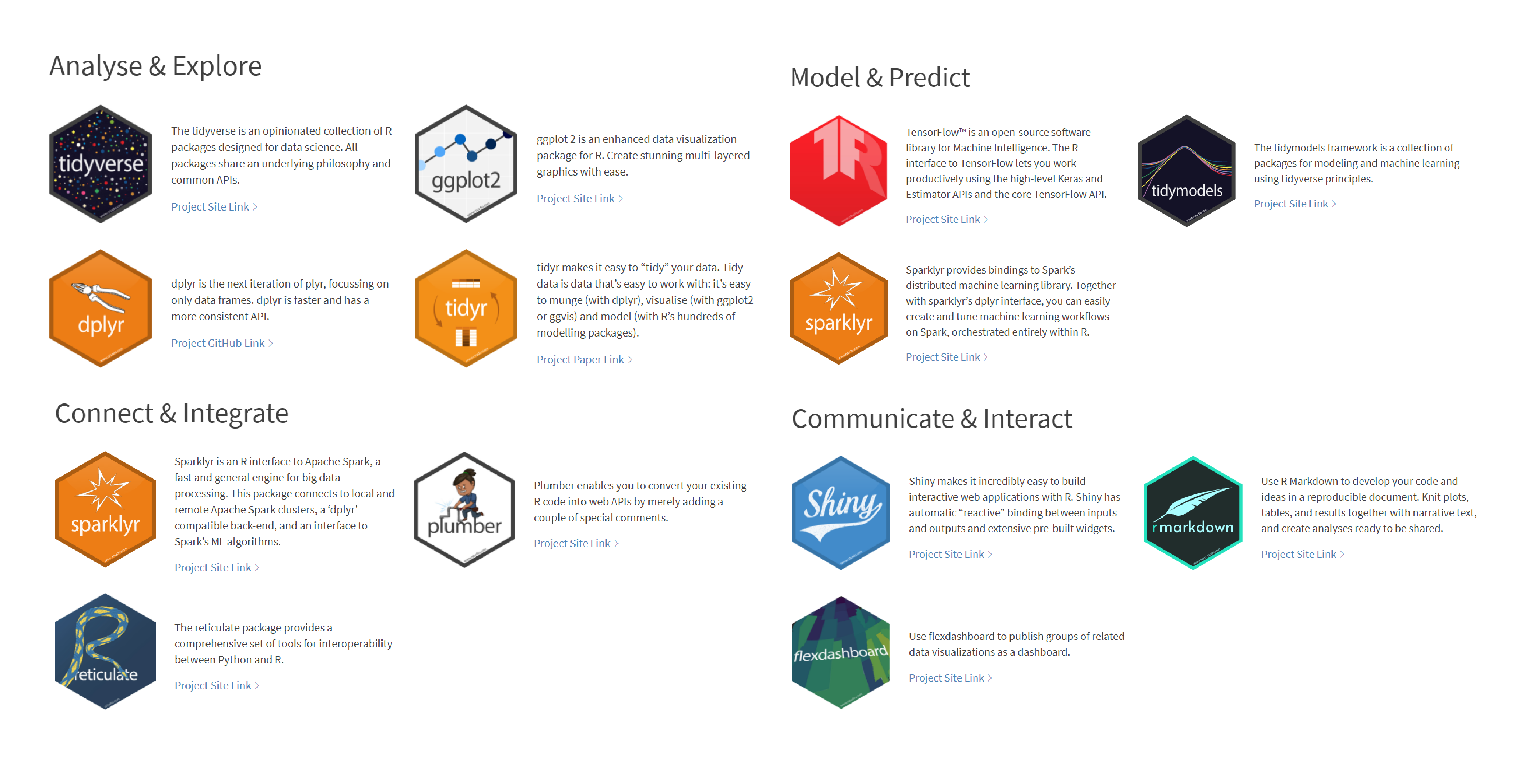
\includegraphics[width=1\linewidth]{2_Abbildungen/pds_2_rstudio_datascienceuniverse} \end{center}
\end{frame}

\begin{frame}{R und RStudio}
\protect\hypertarget{r-und-rstudio-12}{}
\setstretch{1.4}
\large

\textcolor{darkblue}{Lehrmaterialien mit R und RStudio} \vspace{2mm}

\begin{center}
\includegraphics[width=0.8\linewidth]{2_Abbildungen/pds_2_lehrmaterialien} \end{center}
\end{frame}

\begin{frame}{}
\protect\hypertarget{section-4}{}
\large
\vfill
\setstretch{2}

R und RStudio

\textbf{Arithmetik, Logik und Präzedenz}

Variablen

Datenstrukturen

Übungen und Selbstkontrollfragen
\end{frame}

\begin{frame}[fragile]{Arithmetik, Logik und Präzedenz}
\protect\hypertarget{arithmetik-logik-und-pruxe4zedenz}{}
\textcolor{darkblue}{R Konsole als Taschenrechner} \footnotesize
\vspace{1mm}

\begin{Shaded}
\begin{Highlighting}[]
\DecValTok{1}\SpecialCharTok{+}\DecValTok{1}
\end{Highlighting}
\end{Shaded}

\begin{verbatim}
> [1] 2
\end{verbatim}

\begin{Shaded}
\begin{Highlighting}[]
\DecValTok{2}\SpecialCharTok{*}\DecValTok{3}
\end{Highlighting}
\end{Shaded}

\begin{verbatim}
> [1] 6
\end{verbatim}

\begin{Shaded}
\begin{Highlighting}[]
\FunctionTok{sqrt}\NormalTok{(}\DecValTok{2}\NormalTok{)}
\end{Highlighting}
\end{Shaded}

\begin{verbatim}
> [1] 1.41
\end{verbatim}

\begin{Shaded}
\begin{Highlighting}[]
\FunctionTok{exp}\NormalTok{(}\DecValTok{0}\NormalTok{)}
\end{Highlighting}
\end{Shaded}

\begin{verbatim}
> [1] 1
\end{verbatim}

\begin{Shaded}
\begin{Highlighting}[]
\FunctionTok{log}\NormalTok{(}\DecValTok{1}\NormalTok{)}
\end{Highlighting}
\end{Shaded}

\begin{verbatim}
> [1] 0
\end{verbatim}

\begin{itemize}
\item $[1]$ zeigt das erste und einzige Element des Ausgabevektors an
\item Vektoren werden noch im Detail behandelt.
\end{itemize}
\end{frame}

\begin{frame}{Arithmetik, Logik und Präzedenz}
\protect\hypertarget{arithmetik-logik-und-pruxe4zedenz-1}{}
\textcolor{darkblue}{Arithmetische Operatoren} \vspace{4mm}
\setstretch{1.6}

\small
\begin{center}
\begin{tabular}{l|l}
Operator            & Bedeutung                             \\\hline
$+$                 & Addition                              \\
$-$                 & Subtraktion                           \\
$*$                 & Multiplikation                        \\
$/$                 & Division                              \\
\^{} oder $**$      & Potenz                                \\
\%$*$\%             & Matrixmultiplikation                  \\
\%$/$\%             & Ganzzahlige Teilung (5\%$/$\%2 = 2)   \\
\%\%                & Modulo (5\%\%2 = 1)                   \\
\end{tabular}
\end{center}
\vspace{4mm}

\begin{itemize}
\tightlist
\item
  Matrixmultiplikation, Modulo, ganzzahlige Teilung benötigen wir
  zunächst nicht.
\item
  Ganzzahlige Teilung gibt das Resultat der ganzzahligen Teilung an.
\item
  Modulo gibt den ganzzahligen Rest bei ganzzahliger Teilung an.
\end{itemize}
\end{frame}

\begin{frame}{Arithmetik, Logik und Präzedenz}
\protect\hypertarget{arithmetik-logik-und-pruxe4zedenz-2}{}
\setstretch{1.6}

\textcolor{darkblue}{Logische Operatoren} \small

Die Boolesche Algebra und R kennen zwei logische Werte: TRUE und FALSE

Bei Auswertung von Relationsoperatoren ergeben sich logische Werte

\small
\begin{center}
\begin{tabular}{l|l}
Relationsoperator   & Bedeutung                             \\\hline
$==$                & Gleich                                \\
$!=$                & Ungleich                              \\
$<$, $>$            & Kleiner, Größer                       \\
$<=$, $>=$          & Kleiner gleich, Größer gleich         \\
$\vert$             & ODER                                  \\
$\&$                & UND                                   \\
\end{tabular}
\end{center}

\begin{itemize}
\tightlist
\item
  \(<,<=,>,>=\) werden zumeist auf numerische Werte angewendet.
\item
  \(==,!=\) werden zumeist auf beliebige Datenstrukturen angewendet.
\item
  \(\vert\) und \(\&\) werden zumeist auf logische Werte angewendet.
\item
  Die Funktion xor() implementiert das exklusive ODER.
\end{itemize}
\end{frame}

\begin{frame}[fragile]{Arithmetik, Logik und Präzedenz}
\protect\hypertarget{arithmetik-logik-und-pruxe4zedenz-3}{}
\textcolor{darkblue}{Mathematische Funktionen} \setstretch{1.4}

\small
\begin{center}
\begin{tabular}{l|l}
Aufruf              & Bedeutung                                 \\\hline
abs(x)              & Betrag                                    \\
sqrt(x)             & Wurzel                                    \\
ceiling(x)          & Aufrunden (ceiling(2.7) = 3)              \\
floor(x)            & Abrunden (floor(2.7) = 2)                 \\
round(x)            & Mathematisches Runden (round(2.5) = 2)    \\
exp(x)              & Exponentialfunktion                       \\
log(x)              & Logarithmus Funktion                      \\
\end{tabular}
\end{center}

Es handelt sich um eine Auswahl, einen vollständigen Überblick gibt

\begin{Shaded}
\begin{Highlighting}[]
\FunctionTok{names}\NormalTok{(methods}\SpecialCharTok{:::}\NormalTok{.BasicFunsList)}
\end{Highlighting}
\end{Shaded}

R unterscheidet formal nicht zwischen Operatoren und Funktionen

Operatoren können mit der Infix Notation als Funktionen genutzt werden

\begin{Shaded}
\begin{Highlighting}[]
\StringTok{\textasciigrave{}}\AttributeTok{+}\StringTok{\textasciigrave{}}\NormalTok{(}\DecValTok{2}\NormalTok{,}\DecValTok{3}\NormalTok{)            }\CommentTok{\# Infixnotation für 2 + 3}
\end{Highlighting}
\end{Shaded}

\begin{verbatim}
> [1] 5
\end{verbatim}
\end{frame}

\begin{frame}[fragile]{Arithmetik, Logik und Präzedenz}
\protect\hypertarget{arithmetik-logik-und-pruxe4zedenz-4}{}
\textcolor{darkblue}{Operatorpräzedenz} \small

Operatorrangfolge

Regeln der Form ``Punktrechnung vor Strichrechnung'\,'

Vordefinierte Operatorpräzedenz kann durch Klammern überschrieben werden

\begin{Shaded}
\begin{Highlighting}[]
\DecValTok{2} \SpecialCharTok{*} \DecValTok{3} \SpecialCharTok{+} \DecValTok{4}
\end{Highlighting}
\end{Shaded}

\begin{verbatim}
> [1] 10
\end{verbatim}

\begin{Shaded}
\begin{Highlighting}[]
\DecValTok{2} \SpecialCharTok{*}\NormalTok{ (}\DecValTok{3} \SpecialCharTok{+} \DecValTok{4}\NormalTok{)}
\end{Highlighting}
\end{Shaded}

\begin{verbatim}
> [1] 14
\end{verbatim}

Generell gilt

\begin{itemize}
\item
  Operatorrangfolge nicht raten oder folgern, sondern nachschauen!
\item
  Lieber Klammern setzen, als keine Klammern setzen!
\item
  Immer nachschauen, ob Berechnungen die erwarteten Ergebnisse liefern!

\begin{Shaded}
\begin{Highlighting}[]
\NormalTok{?Syntax}
\end{Highlighting}
\end{Shaded}
\end{itemize}
\end{frame}

\begin{frame}[fragile]{Arithmetik, Logik und Präzedenz}
\protect\hypertarget{arithmetik-logik-und-pruxe4zedenz-5}{}
\textcolor{darkblue}{Operatorpräzedenz}

Präzedenz und Ausführungsreihenfolge arithmetischer Operatoren

\small

\begin{center}
\begin{tabular}{l|l}
Operator            & Reihenfolge                               \\\hline
\^{}                & Rechts nach links                         \\
$-$x,$+$x           & Unitäres Vorzeichen, links nach rechts    \\
$*$, $/$            & Links nach Rechts                         \\
$+$, $-$            & Links nach Rechts                         \\
\end{tabular}
\end{center}

Beispiele \footnotesize

\begin{Shaded}
\begin{Highlighting}[]
\DecValTok{2}\SpecialCharTok{\^{}}\DecValTok{2}\SpecialCharTok{\^{}}\DecValTok{3}           \CommentTok{\# 2\^{}(2\^{}3)   = 2\^{}8 = 256}
\NormalTok{(}\DecValTok{2}\SpecialCharTok{\^{}}\DecValTok{2}\NormalTok{)}\SpecialCharTok{\^{}}\DecValTok{3}         \CommentTok{\# (2\^{}2)\^{}3   = 4\^{}3 = 64}
\SpecialCharTok{{-}}\DecValTok{1}\SpecialCharTok{\^{}}\DecValTok{2}            \CommentTok{\# {-}(1\^{}2)    = {-}1}
\NormalTok{(}\SpecialCharTok{{-}}\DecValTok{1}\NormalTok{)}\SpecialCharTok{\^{}}\DecValTok{2}          \CommentTok{\# ({-}1)\^{}2    =  1}
\DecValTok{2}\SpecialCharTok{+}\DecValTok{3}\SpecialCharTok{/}\DecValTok{4}\SpecialCharTok{*}\DecValTok{5}         \CommentTok{\# 2+(3/4)*5 = 2+(0.75*5) = 2+3.75 = 5.75}
\DecValTok{2}\SpecialCharTok{+}\DecValTok{3}\SpecialCharTok{/}\NormalTok{(}\DecValTok{4}\SpecialCharTok{*}\DecValTok{5}\NormalTok{)       }\CommentTok{\# 2+3/(4*5) = 2+3/20 = 2+0.15 = 2.15}
\end{Highlighting}
\end{Shaded}
\end{frame}

\begin{frame}{Arithmetik, Logik und Präzedenz}
\protect\hypertarget{arithmetik-logik-und-pruxe4zedenz-6}{}
\textcolor{darkblue}{Operatorpräzedenz}

\begin{center}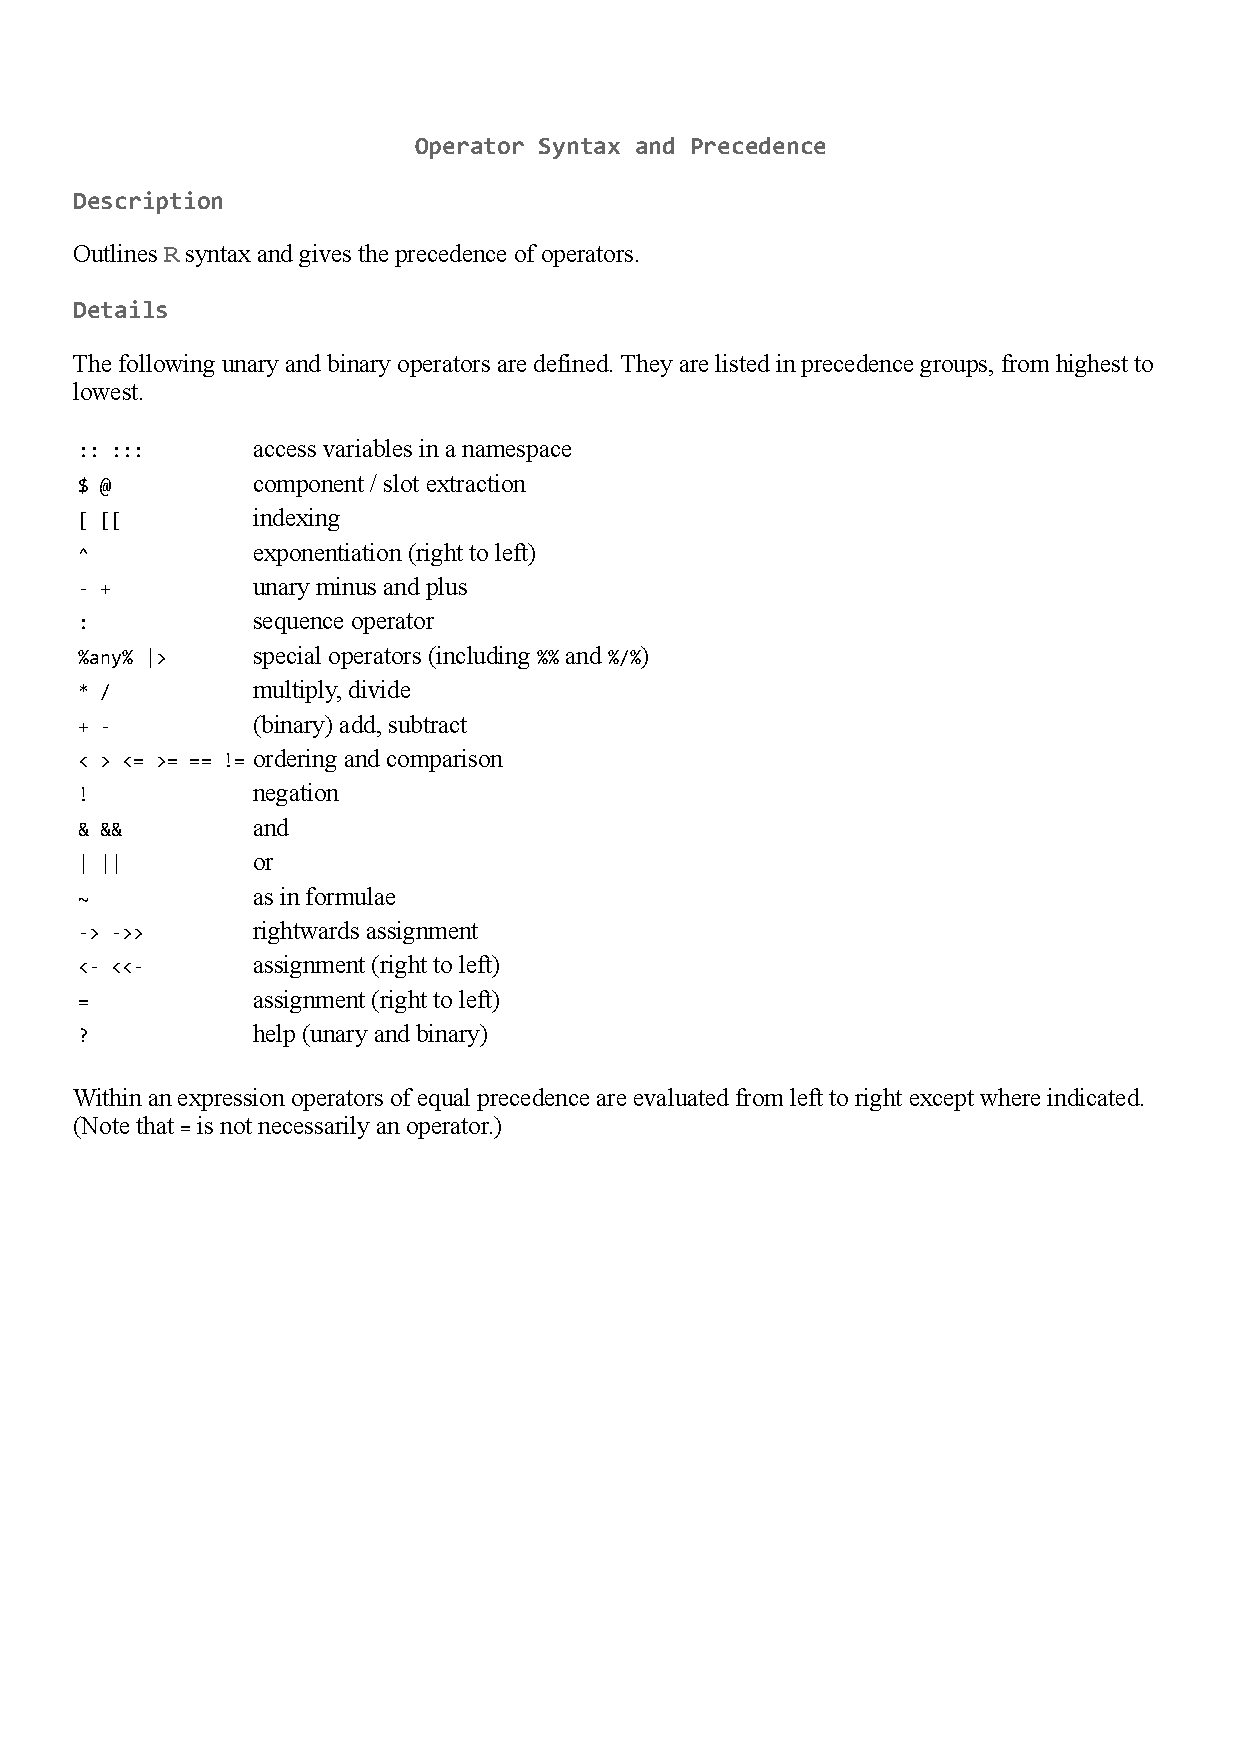
\includegraphics[width=0.7\linewidth]{2_Abbildungen/pds_2_precedence} \end{center}
\end{frame}

\begin{frame}{}
\protect\hypertarget{section-5}{}
\large
\vfill
\setstretch{2}

R und RStudio

Arithmetik, Logik und Präzedenz

\textbf{Variablen}

Datenstrukturen

Übungen und Selbstkontrollfragen
\end{frame}

\begin{frame}{Variablen}
\protect\hypertarget{variablen}{}
\textcolor{darkblue}{Definition} \vspace{5mm}

\small

In der Programmierung ist eine Variable ein abstrakter Behälter für eine
Größe, welche im Verlauf eines Rechenprozesses auftritt. Im Normalfall
wird eine Variable im Quelltext durch einen Namen bezeichnet und hat
eine Adresse im Speicher einer Maschine. Der durch eine Variable
repräsentierte Wert kann -- im Unterschied zu einer Konstante -- zur
Laufzeit des Rechenprozesses verändert werden.

\begin{flushright}
\textit{Wikipedia}
\end{flushright}
\end{frame}

\begin{frame}[fragile]{Variablen}
\protect\hypertarget{variablen-1}{}
\normalsize

\textcolor{darkblue}{Grundlagen} \small

Variablen sind vom Programmierenden benannte Platzhalter für Werte

In 3GL Sprachen wird der Variablentyp durch eine
Initialisierungsanweisung festgelegt:

\begin{Shaded}
\begin{Highlighting}[]
\NormalTok{VAR A }\SpecialCharTok{:}\NormalTok{ INTEGER     }\CommentTok{\# A ist eine Variable vom Typ Integer (ganze Zahl)}
\end{Highlighting}
\end{Shaded}

In 3GL Sprachen wird Variablen durch eine Zuweisungsanweisung ein Wert
zugeschrieben:

\begin{Shaded}
\begin{Highlighting}[]
\NormalTok{A }\SpecialCharTok{:}\ErrorTok{=} \DecValTok{1}              \CommentTok{\# Der Variable A wird der numerische Wert 1 zugewiesen}
\end{Highlighting}
\end{Shaded}

In 4GL Sprachen wie Matlab, Python, R werden Variablen durch Zuweisung
initialisiert:

\begin{Shaded}
\begin{Highlighting}[]
\NormalTok{a }\OtherTok{=} \DecValTok{1}               \CommentTok{\# a ist eine Variable vom Typ double, ihr Wert ist 1\}.}
\end{Highlighting}
\end{Shaded}

Der Zuweisungsbefehl in Matlab und Python ist =, der Zuweisungsbefehl in
R ist \(<-\) oder \(=\)

Offiziell empfohlen für R ist \(<-\), aus Kohärenzgründen benutzen wir
hier \(=\)
\end{frame}

\begin{frame}[fragile]{Variablen}
\protect\hypertarget{variablen-2}{}
\textcolor{darkblue}{Beispiel} \vspace{2mm}

\footnotesize
\justifying

Uta geht ins Schreibwarengeschäft und kauft vier Hefte, zwei Stifte, und
einen Füller. Wie viele Gegenstände kauft Uta insgesamt?

\begin{Shaded}
\begin{Highlighting}[]
\NormalTok{hefte  }\OtherTok{=} \DecValTok{4}      \CommentTok{\# Definition der Variable \textquotesingle{}hefte\textquotesingle{}  und Wertzuweisung 4}
\NormalTok{stifte }\OtherTok{=} \DecValTok{2}      \CommentTok{\# Definition der Variable \textquotesingle{}stifte\textquotesingle{} und Wertzuweisung 2}
\NormalTok{fuller }\OtherTok{=} \DecValTok{1}      \CommentTok{\# Definition der Variable \textquotesingle{}fuller\textquotesingle{} und Wertzuweisung 1}
\end{Highlighting}
\end{Shaded}

Nach Zuweisung existieren die Variablen im Arbeitsspeicher, dem
sogenannten \textit{Workspace}

Die Variablen können jetzt wie Zahlen in Berechnungen genutzt werden

\begin{Shaded}
\begin{Highlighting}[]
\NormalTok{gesamt  }\OtherTok{=}\NormalTok{ hefte }\SpecialCharTok{+}\NormalTok{ stifte }\SpecialCharTok{+}\NormalTok{ fuller                    }\CommentTok{\# Berechnung der Gegenstandsanzahl}
\FunctionTok{print}\NormalTok{(gesamt)}
\end{Highlighting}
\end{Shaded}

\begin{verbatim}
> [1] 7
\end{verbatim}

Ein Heft kostet einen Euro, ein Stift kostet zwei Euro, und ein Füller
kostet 10 Euro. Wie viel Euro muss Uta insgesamt bezahlen?

\begin{Shaded}
\begin{Highlighting}[]
\NormalTok{gesamtpreis }\OtherTok{=}\NormalTok{ hefte}\SpecialCharTok{*}\DecValTok{1} \SpecialCharTok{+}\NormalTok{ stifte}\SpecialCharTok{*}\DecValTok{2} \SpecialCharTok{+}\NormalTok{ fuller}\SpecialCharTok{*}\DecValTok{10}         \CommentTok{\# Berechung des Preises}
\FunctionTok{print}\NormalTok{(gesamtpreis)}
\end{Highlighting}
\end{Shaded}

\begin{verbatim}
> [1] 18
\end{verbatim}

\texttt{print()} gibt Variablenwerte in der R Konsole aus.
\end{frame}

\begin{frame}[fragile]{Variablen}
\protect\hypertarget{variablen-3}{}
\textcolor{darkblue}{Workspace} \vspace{1mm}

\footnotesize

\texttt{ls()} zeigt die existierenden benutzbaren Variablen im
Arbeitsspeicher an

\begin{Shaded}
\begin{Highlighting}[]
\FunctionTok{ls}\NormalTok{()                        }\CommentTok{\# Anzeigen aller Variablennamen im Workspace}
\end{Highlighting}
\end{Shaded}

\begin{verbatim}
> [1] "error_wrap"  "fuller"      "gesamt"      "gesamtpreis"
> [5] "hefte"       "inline_hook" "stifte"
\end{verbatim}

\vspace{2mm}

\texttt{rm()} erlaubt das Löschen von Variablen

\begin{Shaded}
\begin{Highlighting}[]
\FunctionTok{rm}\NormalTok{(gesamtpreis)             }\CommentTok{\# Löschen der Variable Gesamtpreis}
\FunctionTok{ls}\NormalTok{()}
\end{Highlighting}
\end{Shaded}

\begin{verbatim}
> [1] "error_wrap"  "fuller"      "gesamt"      "hefte"      
> [5] "inline_hook" "stifte"
\end{verbatim}

\vspace{2mm}

\texttt{rm(list=ls())} löscht alle Variablen

\begin{Shaded}
\begin{Highlighting}[]
\FunctionTok{rm}\NormalTok{(}\AttributeTok{list =} \FunctionTok{ls}\NormalTok{())             }\CommentTok{\# Löschen aller Variablen}
\FunctionTok{ls}\NormalTok{()}
\end{Highlighting}
\end{Shaded}

\begin{verbatim}
> character(0)
\end{verbatim}
\end{frame}

\begin{frame}{Variablen}
\protect\hypertarget{variablen-4}{}
\textcolor{darkblue}{Workspace} \vfill

\begin{center}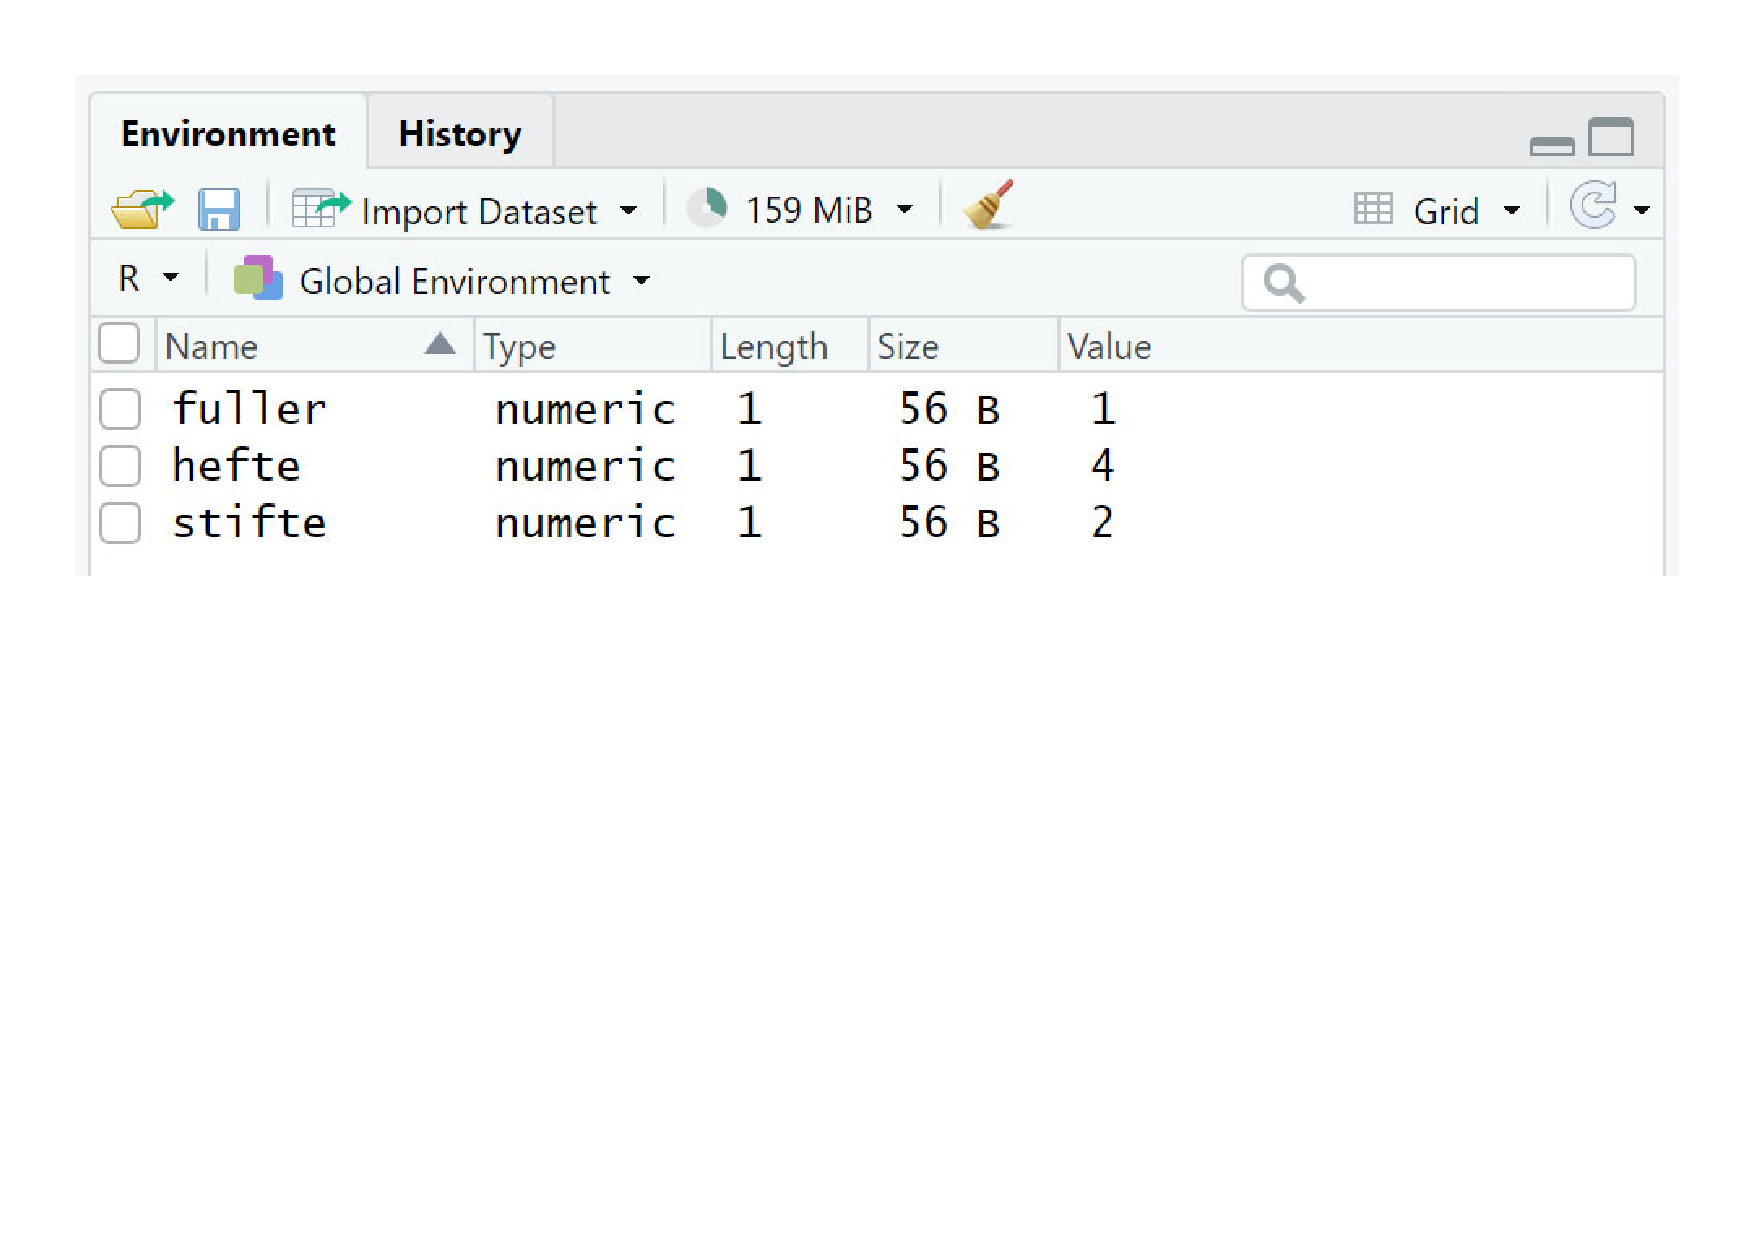
\includegraphics[width=0.9\linewidth]{2_Abbildungen/pds_2_workspace} \end{center}
\vfill
\end{frame}

\begin{frame}{Variablen}
\protect\hypertarget{variablen-5}{}
\setstretch{1.6}

\textcolor{darkblue}{Variablennamen}

\vspace{2mm}

Zulässige Variablennamen

\ldots{} bestehen aus Buchstaben, Zahlen, Punkten (.) und Unterstrichen
(\_)

\ldots{} beginnen mit einem Buchstaben oder . nicht gefolgt von einer
Zahl

\ldots{} dürfen keine reserverd words wie \textcolor{blue}{for},
\textcolor{blue}{if}, \textcolor{blue}{NaN}, usw. sein (\(>\)?reserved)

\ldots{} werden unter ?make.names() beschrieben

Sinnvolle Variablennamen

\ldots{} sind kurz (\(\approx\) 1 bis 7 Zeichen) und aussagekräftig

\ldots{} bestehen nur aus Kleinbuchstaben und Unterstrichen
\end{frame}

\begin{frame}[fragile]{Variablen}
\protect\hypertarget{variablen-6}{}
\textcolor{darkblue}{Variablenrepräsentation $\vert$ Binding}
\vspace{1mm} \footnotesize \setstretch{0.5}

\begin{Shaded}
\begin{Highlighting}[]
\NormalTok{x }\OtherTok{=} \DecValTok{1}
\end{Highlighting}
\end{Shaded}

Intuitiv wird eine Variable genannt x mit dem Wert 1 erzeugt.

De-facto geschehen zwei Dinge:

\begin{enumerate}
\tightlist
\item
  R erzeugt ein Objekt (Vektor mit Wert 1) mit Speicheradresse
  `lobstr::obj\_addr(x).
\item
  R verbindet dieses Objekt mit dem Namen x, der das Objekt im Speicher
  referenziert.
\end{enumerate}

\begin{center}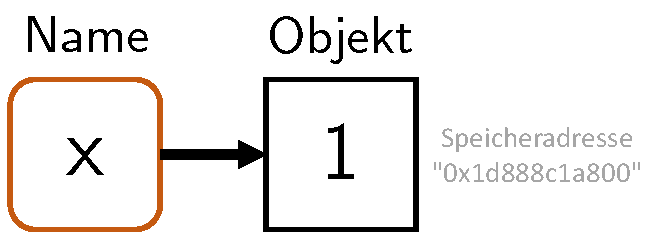
\includegraphics[width=0.22\linewidth]{2_Abbildungen/pds_2_binding_1} \end{center}
\vspace{1mm}

\begin{Shaded}
\begin{Highlighting}[]
\NormalTok{y }\OtherTok{=}\NormalTok{ x}
\end{Highlighting}
\end{Shaded}

Intuitiv wird eine Variable genannt y mit Wert gleich dem Wert von x
erzeugt.

De-facto wird ein neuer Name y erzeugt, der dasselbe Objekt referenziert
wie x:

\begin{center}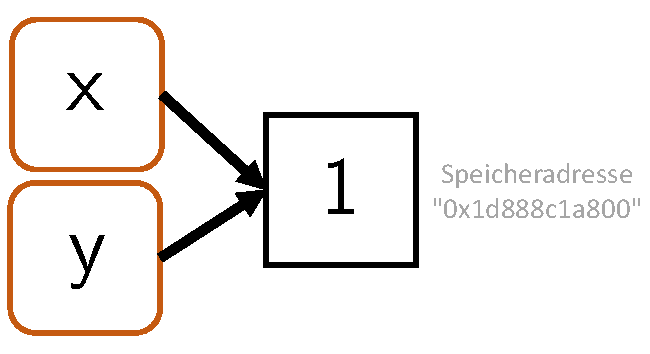
\includegraphics[width=0.22\linewidth]{2_Abbildungen/pds_2_binding_2} \end{center}
\vspace{1mm}

Man überzeuge sich mit \texttt{lobstr::obj\_addr(x)} und
`lobstr::obj\_addr(y).

Das Objekt (Vektor mit Wert 1) wird nicht kopiert, R spart
Arbeitsspeicher.
\end{frame}

\begin{frame}[fragile]{Variablen}
\protect\hypertarget{variablen-7}{}
\textcolor{darkblue}{Variablenrepräsentation $\vert$ Copy-on-modify}
\vspace{2mm} \small

\begin{Shaded}
\begin{Highlighting}[]
\NormalTok{x }\OtherTok{=} \DecValTok{1}       \CommentTok{\# Objekt (0x74b) erzeugt, x referenziert Speicheradresse  des Objektes}
\NormalTok{y }\OtherTok{=}\NormalTok{ x       }\CommentTok{\# y referenziert dieselbe Speicheradresse wie x (0x74b)}
\NormalTok{y }\OtherTok{=} \DecValTok{3}       \CommentTok{\# y modifiziert, modifizierte Kopie (0xcd2) wird gespeichert}
\NormalTok{y           }\CommentTok{\# y referenziert jetzt (0xcd2)}
\end{Highlighting}
\end{Shaded}

\begin{verbatim}
> [1] 3
\end{verbatim}

\begin{Shaded}
\begin{Highlighting}[]
\NormalTok{x           }\CommentTok{\# x referenziert weiterhin (0x74b)}
\end{Highlighting}
\end{Shaded}

\begin{verbatim}
> [1] 1
\end{verbatim}

\begin{center}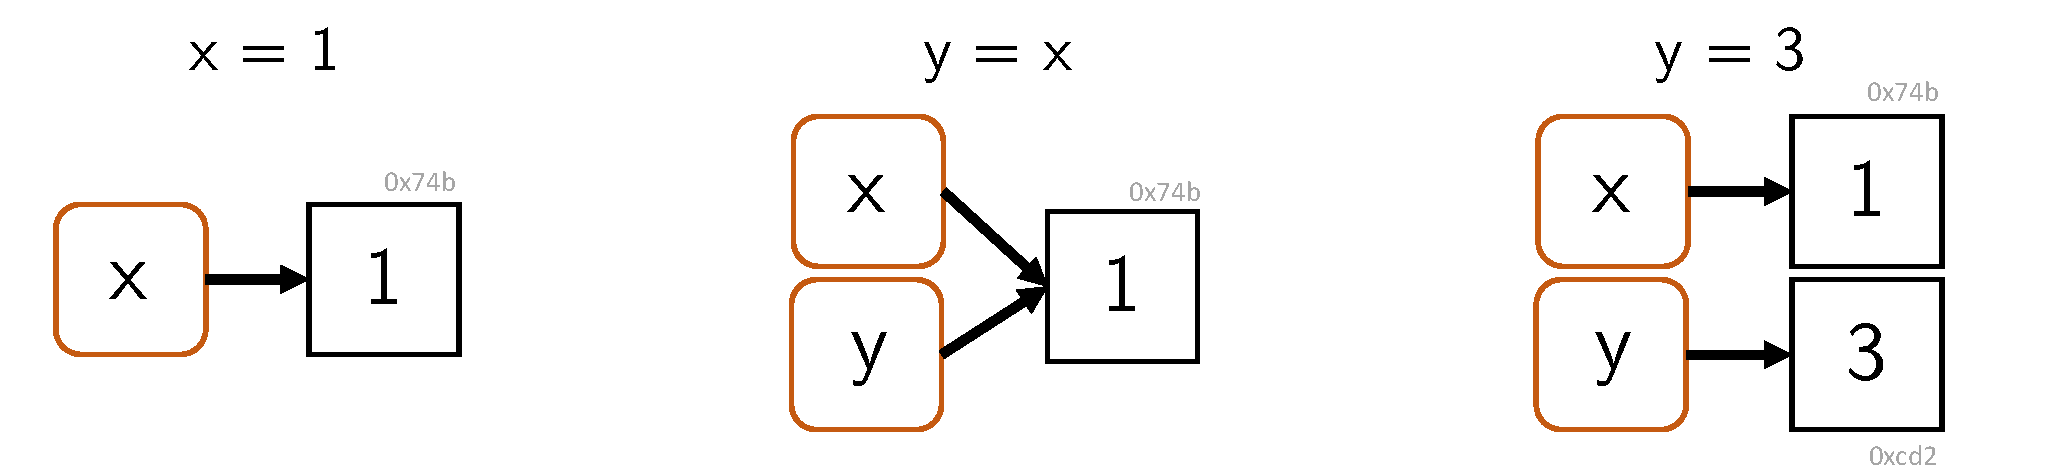
\includegraphics[width=0.7\linewidth]{2_Abbildungen/pds_2_copy_on_modify} \end{center}

R Objekte sind \textit{immutable}, können also nicht verändert werden.
\end{frame}

\begin{frame}[fragile]{Variablen}
\protect\hypertarget{variablen-8}{}
\textcolor{darkblue}{Variablenrepräsentation $\vert$ Copy-on-modify}
\vspace{2mm} \small \setstretch{2.5}

Zur Immutability gibt allerdings zwei Ausnahmen, genannt
\textit{Modifications-in-place}

\begin{enumerate}
\item
  Objekte mit nur einem gebundenem Namen werden in-place modifiziert

  \begin{itemize}
  \item
    \footnotesize Dieses Verhalten ist allerdings nur in R, nicht
    innerhalb RStudios reproduzierbar.

\begin{Shaded}
\begin{Highlighting}[]
\NormalTok{x }\OtherTok{=} \DecValTok{1}         \CommentTok{\# Objekt (0x74b) erzeugt, x referenziert Speicheradresse des Objektes}
\NormalTok{x[}\DecValTok{1}\NormalTok{] }\OtherTok{=} \DecValTok{2}  \CommentTok{\# Objekt (0x74b) veraendert}
\end{Highlighting}
\end{Shaded}
  \end{itemize}
\end{enumerate}

\small

\begin{enumerate}
\setcounter{enumi}{1}
\tightlist
\item
  Environments werden in-place modifiziert (\(\rightarrow\) Environments
  und Funktionen).
\end{enumerate}
\end{frame}

\begin{frame}[fragile]{Variablen}
\protect\hypertarget{variablen-9}{}
\textcolor{darkblue}{Variablenrepräsentation $\vert$ Unbinding und Carbage Collection}
\small

Copy-on-modify gilt auch in umgekehrter Reihenfolge

\footnotesize

\begin{Shaded}
\begin{Highlighting}[]
\NormalTok{x }\OtherTok{=} \DecValTok{1}       \CommentTok{\# Objekt (0x74b) erzeugt, x referenziert Speicheradresse  des Objektes}
\NormalTok{y }\OtherTok{=}\NormalTok{ x       }\CommentTok{\# y referenziert dieselbe Speicheradresse wie x (0x74b)}
\NormalTok{x }\OtherTok{=} \DecValTok{3}       \CommentTok{\# Ein neues Objekt (0x2a08) wird erzeugt, x referenziert (0x2a08)}
\NormalTok{y           }\CommentTok{\# y referenziert weiterhin  Objekt (0x74b)}
\end{Highlighting}
\end{Shaded}

\begin{verbatim}
> [1] 1
\end{verbatim}

\begin{center}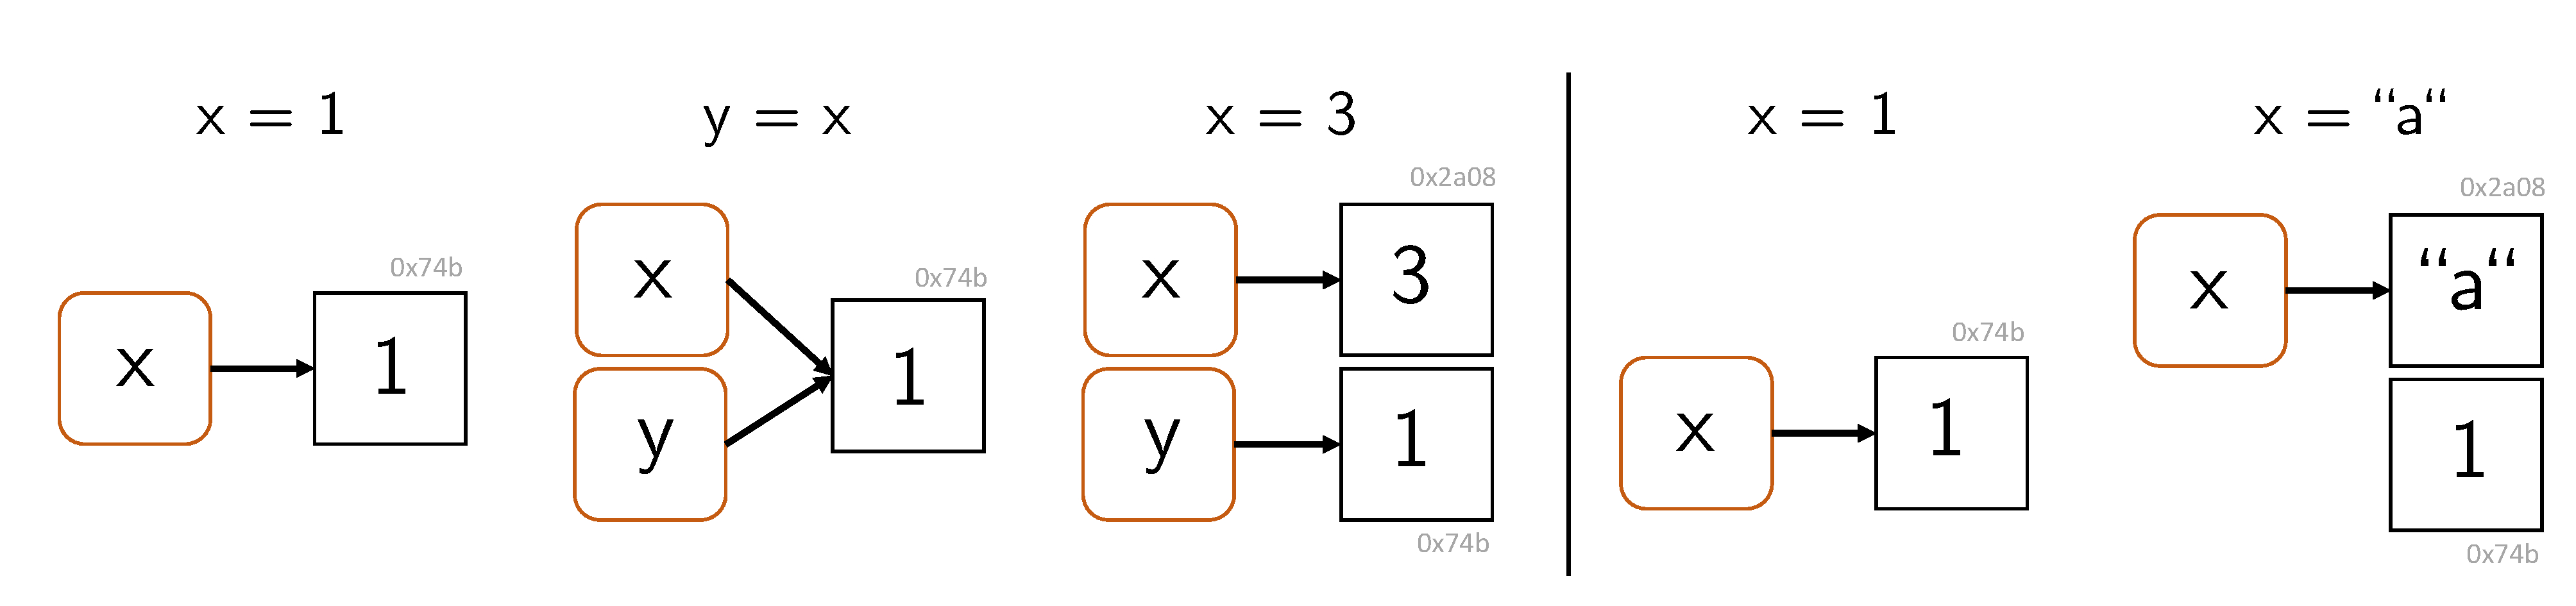
\includegraphics[width=0.56\linewidth]{2_Abbildungen/pds_2_unbinding} \end{center}
\vspace{-2mm}
\small

Unbinding \footnotesize

\begin{Shaded}
\begin{Highlighting}[]
\NormalTok{x }\OtherTok{=} \DecValTok{1}       \CommentTok{\#  x referenziert Objekt (0x74b)}
\NormalTok{x }\OtherTok{=} \StringTok{"a"}     \CommentTok{\#  x referenziert Objekt (0x2a08), Objekt (0x74b) jetzt ohne Referenz}
\end{Highlighting}
\end{Shaded}

\small

Carbage collection \footnotesize

\begin{itemize}
\tightlist
\item
  Nicht referenzierte Objekte im Arbeitsspeicher werden automatisch
  gelöscht.
\item
  Das Löschen geschieht meist erst dann, wenn es wirklich nötig ist.
\item
  Es ist nicht nötig, aktiv die Garbage Collection Funktion
  \texttt{gc()} zu benutzen.
\end{itemize}
\end{frame}

\begin{frame}{}
\protect\hypertarget{section-6}{}
\large
\vfill
\setstretch{2}

R und RStudio

Arithmetik, Logik und Präzedenz

Variablen

\textbf{Datenstrukturen}

Übungen und Selbstkontrollfragen
\end{frame}

\begin{frame}[fragile]{Datenstrukturen}
\protect\hypertarget{datenstrukturen}{}
\textcolor{darkblue}{Klassische Datenstrukturen einer 3GL Programmiersprache}

\small

\textcolor{darkblue}{Fundamentale Datenstrukturen}

\begin{itemize}
\tightlist
\item
  Vordefiniert innerhalb der Programmiersprache
\item
  Logische Werte (logical): TRUE, FALSE
\item
  Ganze Zahlen (integer): int8 (-128,\ldots,127), int16 (--32768,\ldots,
  32767)
\item
  Gleitkommazahlen (single, double): 1.23456, 12.3456, 123.456, \ldots{}
\item
  Zeichen (character):
  \texttt{a\textquotesingle{}\textquotesingle{},}b'`,
  \texttt{c\textquotesingle{}\textquotesingle{},}!''
\item
  Datentyp-spezifische assoziierte Operationen

  \begin{itemize}
  \tightlist
  \item
    \small AND, OR (logical) +, - (integer) +,-,*, / (single),
    Zeichenkonkatenation (character)
  \end{itemize}
\end{itemize}

\textcolor{darkblue}{Zusammengesetzte Datenstrukturen}

\begin{itemize}
\tightlist
\item
  Vordefinierte Container zur Zusammenfassung mehrerer Variablen
  gleichen Datentyps
\item
  Zum Beispiel Vektoren, Listen, Arrays, Matrizen, \ldots{}
\item
  Container-spezifische Operationen (Z.B. Vektorindizierung,
  Matrixmultiplikation, \ldots)
\end{itemize}

\textcolor{darkblue}{Selbstdefinierte Datenstrukturen}

\begin{itemize}
\tightlist
\item
  Definition eigener Datenstrukturen aus vordefinierten Datenstrukturen
  und Containern
\item
  Definition eigener Operationen
\end{itemize}
\end{frame}

\begin{frame}{Datenstrukturen}
\protect\hypertarget{datenstrukturen-1}{}
\textcolor{darkblue}{Datenstrukturenkennenlernen beim Erlernen einer Programmiersprache}

\small

\textcolor{darkblue}{Fundamentale Datenstrukturen}

\begin{itemize}
\tightlist
\item
  Welche fundamentalen Datenstrukturen bietet die Sprache an?
\item
  Welche Operationen darauf sind bereits definiert?
\item
  Wie lautet die Syntax zur Definition einer Variable eines
  fundamentalen Datentyps?
\item
  Wie lautet die Syntax, um vordefinierte Operationen aufzurufen?
\end{itemize}

\textcolor{darkblue}{Zusammengesetzte Datenstrukturen}

\begin{itemize}
\tightlist
\item
  Welche Container und zugehörige Operationen bietet die
  Programmiersprache?
\item
  Wie lautet die Syntax zum Umgang mit einem Containers?
\end{itemize}

\textcolor{darkblue}{Selbstdefinierte Datenstrukturen}

\begin{itemize}
\tightlist
\item
  Wie erzeugt man selbstdefinierte Datenstrukturen und zugehörige
  Operationen?
\item
  Wie lautet die Syntax zum Umgang mit einer selbstdefinierten
  Datenstruktur?
\end{itemize}
\end{frame}

\begin{frame}{Datenstrukturen}
\protect\hypertarget{datenstrukturen-2}{}
\setstretch{1.8}

\textcolor{darkblue}{Organisation von Daten in R} \vspace{1mm}

Alles, was in R vorkommt, ist ein \textbf{Objekt} \vspace{1mm}

Jedem Objekt kann eindeutig zugeordnet werden

\begin{itemize}
\item
  ein \textbf{Modus}

  \begin{itemize}
  \tightlist
  \item
    Atomar \(\,\,\vert\) Komponenten sind vom gleichen Datentyp.
  \item
    Rekursiv \(\vert\) Komponenten können von unterschiedlichem Datentyp
    sein.
  \end{itemize}
\item
  eine \textbf{Länge}
\item
  optional weitere \textbf{Attribute}
\end{itemize}
\end{frame}

\begin{frame}{Datenstrukturen}
\protect\hypertarget{datenstrukturen-3}{}
\setstretch{1.8}

\textcolor{darkblue}{Organisation von Daten in R} \vspace{1mm}

Alles, was in R vorkommt, ist ein \textbf{Objekt} \vspace{5mm}

\begin{center}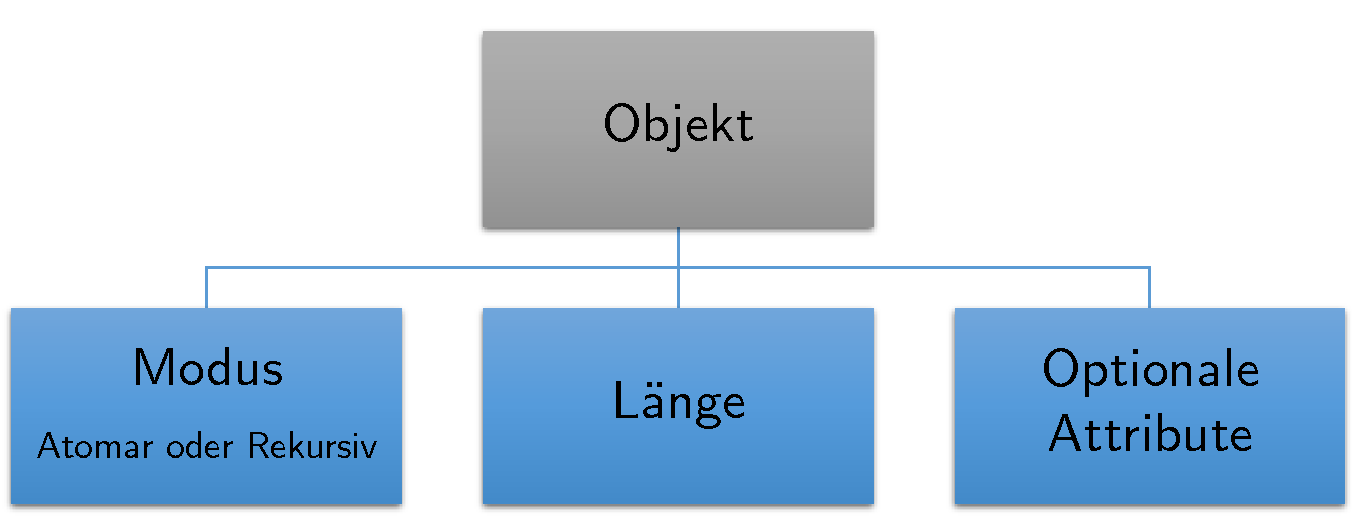
\includegraphics[width=0.8\linewidth]{2_Abbildungen/pds_2_r_objektstruktur} \end{center}
\end{frame}

\begin{frame}{Datenstrukturen}
\protect\hypertarget{datenstrukturen-4}{}
\textcolor{darkblue}{Übersicht der R Datentypen} \small \setstretch{1.8}
\vspace{5mm}

\begin{center}
\begin{tabular}{l|l}
Datentyp
& Erläuterung
\\\hline
logical
& Die beiden logischen Werte TRUE und FALSE
\\
double
&
Gleitkommazahlen
\\
integer
& Ganze Zahlen
\\
complex
& Komplexe Zahlen, hier nicht weiter besprochen
\\
character
& Zeichen und Zeichenketten (strings), 'x' oder ``Hallo Welt!''
\\
raw
& Bytes, hier nicht weiter besprochen
\\
\end{tabular}
\end{center}
\vspace{2mm}

Double und integer werden zusammen auch als numeric bezeichnet.

Viele weitere Typen, hier relevant sind \textbf{logical},
\textbf{double}, \textbf{integer}, \textbf{character}.
\end{frame}

\begin{frame}[fragile]{Datenstrukturen}
\protect\hypertarget{datenstrukturen-5}{}
\setstretch{0.8}
\vspace{1mm}

\textcolor{darkblue}{Übersicht der R Datentypen} \footnotesize

Automatische Festlegung von Datentypen durch Zuweisung \vspace{1mm}

\begin{Shaded}
\begin{Highlighting}[]
\NormalTok{b }\OtherTok{=} \ConstantTok{TRUE}                    \CommentTok{\# logical}
\NormalTok{x }\OtherTok{=} \FloatTok{2.5}                     \CommentTok{\# double}
\NormalTok{y }\OtherTok{=}\NormalTok{ 1L                      }\CommentTok{\# (long) integer}
\NormalTok{c }\OtherTok{=} \StringTok{\textquotesingle{}a\textquotesingle{}}                     \CommentTok{\# character}
\end{Highlighting}
\end{Shaded}

Testen von Datentypen durch \texttt{typeof()} \vspace{1mm}

\begin{Shaded}
\begin{Highlighting}[]
\FunctionTok{typeof}\NormalTok{(b)}
\end{Highlighting}
\end{Shaded}

\begin{verbatim}
> [1] "logical"
\end{verbatim}

\begin{Shaded}
\begin{Highlighting}[]
\FunctionTok{typeof}\NormalTok{(x)}
\end{Highlighting}
\end{Shaded}

\begin{verbatim}
> [1] "double"
\end{verbatim}

\begin{Shaded}
\begin{Highlighting}[]
\FunctionTok{typeof}\NormalTok{(y)}
\end{Highlighting}
\end{Shaded}

\begin{verbatim}
> [1] "integer"
\end{verbatim}

\begin{Shaded}
\begin{Highlighting}[]
\FunctionTok{typeof}\NormalTok{(c)}
\end{Highlighting}
\end{Shaded}

\begin{verbatim}
> [1] "character"
\end{verbatim}

Testen von Datetypen durch \texttt{is.*()} \vspace{1mm}

\begin{Shaded}
\begin{Highlighting}[]
\FunctionTok{is.logical}\NormalTok{(x)}
\end{Highlighting}
\end{Shaded}

\begin{verbatim}
> [1] FALSE
\end{verbatim}

\begin{Shaded}
\begin{Highlighting}[]
\FunctionTok{is.double}\NormalTok{(x)}
\end{Highlighting}
\end{Shaded}

\begin{verbatim}
> [1] TRUE
\end{verbatim}
\end{frame}

\begin{frame}{Datenstrukturen}
\protect\hypertarget{datenstrukturen-6}{}
\setstretch{2}

\textcolor{darkblue}{Übersicht atomare Datenstrukturen in R}
\vspace{3mm}

\begin{center}
\begin{tabular}{l|l}
Datenstruktur
& Erläuterung
\\\hline

Vektor
& Container von indizierte Komponenten identischen Typs
\\

Matrix
& Interpretation eines Vektors als zweidimensionaler Container
\\

Array
&  Interpretation eines Vektors als mehrdimensionaler Container

\end{tabular}
\end{center}
\vspace{3mm}

\(\Rightarrow\) (3) Vektoren, Matrizen, Arrays
\end{frame}

\begin{frame}{Datenstrukturen}
\protect\hypertarget{datenstrukturen-7}{}
\setstretch{2}

\textcolor{darkblue}{Übersicht rekursive Datenstrukturen in R}
\vspace{3mm}

\begin{center}
\begin{tabular}{l|l}
Datenstruktur
& Erläuterung
\\\hline

Liste
& Container von indizierten Komponenten beliebigen Datentyps
\\
& Insbesondere auch rekursive Struktur, z.B. Liste von Listen
\\

Dataframe
& Symbiose aus Liste und Matrix
\\
& Jede Komponente ist Vektor beliebigen Datentyps identischer Länge
\\
\end{tabular}
\end{center}
\vspace{3mm}

\(\Rightarrow\) (4) Listen und Dataframes
\end{frame}

\begin{frame}{}
\protect\hypertarget{section-7}{}
\large
\vfill
\setstretch{2}

R und RStudio

Arithmetik, Logik und Präzedenz

Variablen

Datenstrukturen

\textbf{Übungen und Selbstkontrollfragen}
\end{frame}

\begin{frame}{Übungen und Selbstkontrollfragen}
\protect\hypertarget{uxfcbungen-und-selbstkontrollfragen}{}
\footnotesize

\begin{enumerate}
\tightlist
\item
  Installieren Sie R und RStudio auf Ihrem Rechner.
\item
  Führen Sie die Befehlssequenz auf Folie
  \textcolor{blue}{R Skripte $\vert$ Executing and Editing Code} aus.
\item
  Dokumentieren Sie die in dieser Einheit eingeführten R Befehle in
  einem kommentierten R Skript.
\item
  Erläutern Sie den Begriff der Operatorpräzedenz.
\item
  Definieren Sie den Begriff der Variable im Kontext der Programmierung.
\item
  Erläutern Sie die Begriffe Initialisierungsanweisung und
  Zuweisungsanweisung für Variablen.
\item
  Erläutern Sie den Begriff Workspace.
\item
  Geben Sie jeweils ein Beispiel für einen zulässigen und einen
  unzulässigen Variablennamen in R.
\item
  Erläutern Sie die Prozesse, die R im Rahmen einer Zuweisungsanweisung
  der Form x = 1 durchführt.
\item
  Erläutern Sie den Begriffe Copy-on-modify und Modify-in-place.
\item
  Diskutieren Sie die klassischen Datenstrukturen einer 3GL
  Programmiersprache.
\item
  Diskutieren Sie die Organisation von Datenstrukturen in R.
\item
  Wodurch unterscheiden sich eine atomare und ein rekursive
  Datenstruktur in R?
\item
  Nennen und erläutern Sie vier zentrale Datentypen in R.
\item
  Nennen und erläutern Sie vier zentrale atomare Datenstrukturen in R.
\item
  Nennen und erläutern Sie zwei zentrale rekursive Datenstrukturen in R.
\end{enumerate}
\end{frame}

\begin{frame}{References}
\protect\hypertarget{references}{}
\footnotesize

\hypertarget{refs}{}
\begin{CSLReferences}{1}{0}
\leavevmode\hypertarget{ref-becker_new_1988}{}%
Becker, Richard A., John M. Chambers, and Allen Reeve Wilks. 1988.
\emph{The New {S} Language: A Programming Environment for Data Analysis
and Graphics}. Reprint. {London}: {Chapman \& Hall}.

\leavevmode\hypertarget{ref-ihaka_language_1996}{}%
Ihaka, Ross, and Robert Gentleman. 1996. {``R: {A Language} for {Data
Analysis} and {Graphics}.''} \emph{Journal of Computational and
Graphical Statistics} 5 (3): 2999--2314.

\end{CSLReferences}
\end{frame}

\end{document}
